% -*- root: 00-main.tex -*-
\section{Methods}
\label{sec:methods}
%
Let $\gammaset_R = \{\Gamma_m: m \in \mathbb{N}, m \leq N_c\}$ be the set of $N_c$ surfaces
  extracted from the undistorted \gls*{t1} image (the reference space $R$).
We reformulate the segmentation of the distorted \gls*{dmri} images (the moving space $M$)
  as a registration problem where we look for an underlying deformation field $U$, such that 
  the structures in $R$ defined by $\gammaset_R$ optimally align with their corresponding
  structures in $M$:

  \begin{align}
  U\colon R \subset \mathbb{R}^n &\to M \subset \mathbb{R}^n \notag\\
  \vec{r} &\mapsto \vec{r}' =\vec{r}+\vec{u}(\vec{r}),
  \label{eq:transform}
  \end{align}
%
  where $\vec{r}$ denotes a position in $R$, $\vec{r}'$ is
  its corresponding location in $M$, and $n$ the dimensionality of images.
Finally, $\vec{u} = \vec{u}(\vec{r})$ is the displacement of every point with respect
  to the reference domain.

\subsection{Cost-function derivation}\label{sec:methods_map}
%
In a Bayesian framework for registration \citep{wyatt_map_2003,pohl_bayesian_2006,gass_simultaneous_2014},
  the mappings $U$ in \eqref{eq:transform} are
  evaluated based on their posterior probability given the observed data
  $M$.
Let $\omegaset = \{\Omega_l: l \in \mathbb{N}, l \leq N_L\}$ be the set of $N_L$ competing regions in
  which $M$ is partitioned by the projection of $\gammaset_R$.
Using the Bayes' rule, the posterior likelihood is computed as:

  \begin{equation}
  P(U \mid M, \omegaset ) = \frac{P(M \mid U,\omegaset )\, P(U)}{P(M)},
  \label{eq:bayes_rule}
  \end{equation}
%
  where $P(M \mid U,\omegaset)$ is the data-likelihood.
As $\omegaset$ are mapped by $U$, we simplify
  $P(U, \omegaset) = P(U) \implies P(M \mid U,\omegaset) = P(M \mid U)$.

The best estimate $\hat{U}$ then fulfills the maximum a posteriori criterium
  \citep{bishop_pattern_2006}, and aligns $\gammaset_R$ into $M$.
First, we assume independence between pixels, and thus break down the
  global data likelihood into a product of pixel-wise conditional probabilities:

  \begin{equation}
  P(M \mid U) = \underset{l}{\prod} \underset{\vec{r}\in \Omega_l}{\prod}
    P\left( \vec{f}' \mid U \right),
  \label{eq:bayes_aposteriori}
  \end{equation}
%
  where $\vec{f}' = M(\vec{r}')$ is the feature vector at the displaced
  position $\vec{r}'$ \eqref{eq:transform} in the moving image.
For convenience, and because it has been shown to be an appropriate approximation
  \citep{leemput_automated_1999,cuadra_comparison_2005}, we introduce two assumptions for each
  region $\Omega_l$:
  1) the features are i.i.d.; and 2) they can be modeled by multivariate normal
  distributions with parameters $\lbrace \boldsymbol{\mu}_l, \boldsymbol{\Sigma}_{l} \rbrace$
  for each region $\Omega_l$:

 	\begin{align}
  P( M \mid U) &= \underset{l}{\prod} \underset{\vec{r} \in \Omega_l}{\prod}
  \mathcal{N} ( \vec{f} \mid \boldsymbol{\mu}_l, \boldsymbol{\Sigma}_{l} ) = % \notag\\ &=
  \underset{l}{\prod} \underset{\vec{r} \in \Omega_l}{\prod} \frac{1}{ \sqrt{(2\pi)^{C}\,\left|\boldsymbol{\Sigma}_{l}\right|}}\,{e^{\left(-\frac{1}{2}
  \mdist{f'}{l} \right)}},
  \label{eq:pdf}
  \end{align}
%
  using $\mdist{f}{l}$ to denote the squared \emph{Mahalanobis distance} of $\vec{f}$ with respect
  to the descriptors of region $l$ as
  $\mdist{f}{l} = (\vec{f} - \boldsymbol{\mu}_l)^T \, {\boldsymbol{\Sigma}_l}^{-1} \, (\vec{f} - \boldsymbol{\mu}_l)$.
$C$ is the number of channels comprised in the image $M$.
In fact, the projection of $\gammaset_R$ onto $M$ is an implicit segmentation model, for which
  the covariance matrix $\boldsymbol{\Sigma}_l$ of each region is minimized.

The smoothness of the resulting displacements field is induced by a Thikonov regularization
  prior:

  \begin{align}
  P(U) = \underset{\vec{r}}{\prod}\, p(\vec{u}) &=
  \underset{\vec{r}}{\prod}\, p_0(\vec{u}) \, p_1(\vec{u}), \text{ with} \\
  p_0(\vec{u}) &= \mathcal{N}( \vec{u} \mid 0, \mathbf{A}^{-1}), \notag\\
  p_1(\vec{u}) &= \mathcal{N}(  \nabla \vec{u} \mid 0, \mathbf{B}^{-1}),
  \label{eq:thikonov}
  \end{align}
%
  imposing that the distortion and its gradient have zero
  mean and variance governed by the matrices $\mathbf{A}$ and $\mathbf{B}$.
Finally, the maximum a posteriori problem is adapted into a variational one where we look for
  the minimum of an energy functional, by applying $E(\vec{u}) = -\log P(U)$:

  \begin{align}
  E(\vec{u}) &= -\log \underset{l}{\prod}
  \underset{\vec{r} \in \Omega_l}{\prod}
  \mathcal{N} \left( \vec{f}' \mid \boldsymbol{\mu}_l, \boldsymbol{\Sigma}_l \right)\,p_0( \vec{u})\,p_1( \vec{u}) = \notag\\ &=
  \const + \underset{l}{\sum} \int_{\Omega_l} \mdist{f'}{l} \,d\vec{r} \, + % \notag\\ &+
  \int_{\Omega} \frac12 \left[ \vec{u}^T \mathbf{A} \vec{u} + (\nabla \vec{u})^T \mathbf{B} (\nabla \vec{u}) \right] \,d\vec{r}.
  \label{eq:energy}
  \end{align}
%
This expression is dual of the Mumford-Shah functional corresponding
  to a framework of \acrlong*{acwe} \citep{chan_active_2001}
  with the corresponding anisotropic regularization term of \cite{nagel_investigation_1986}.


\subsection{Numerical Implementation}
\label{sec:numerical_implementation}

\begin{figure}
	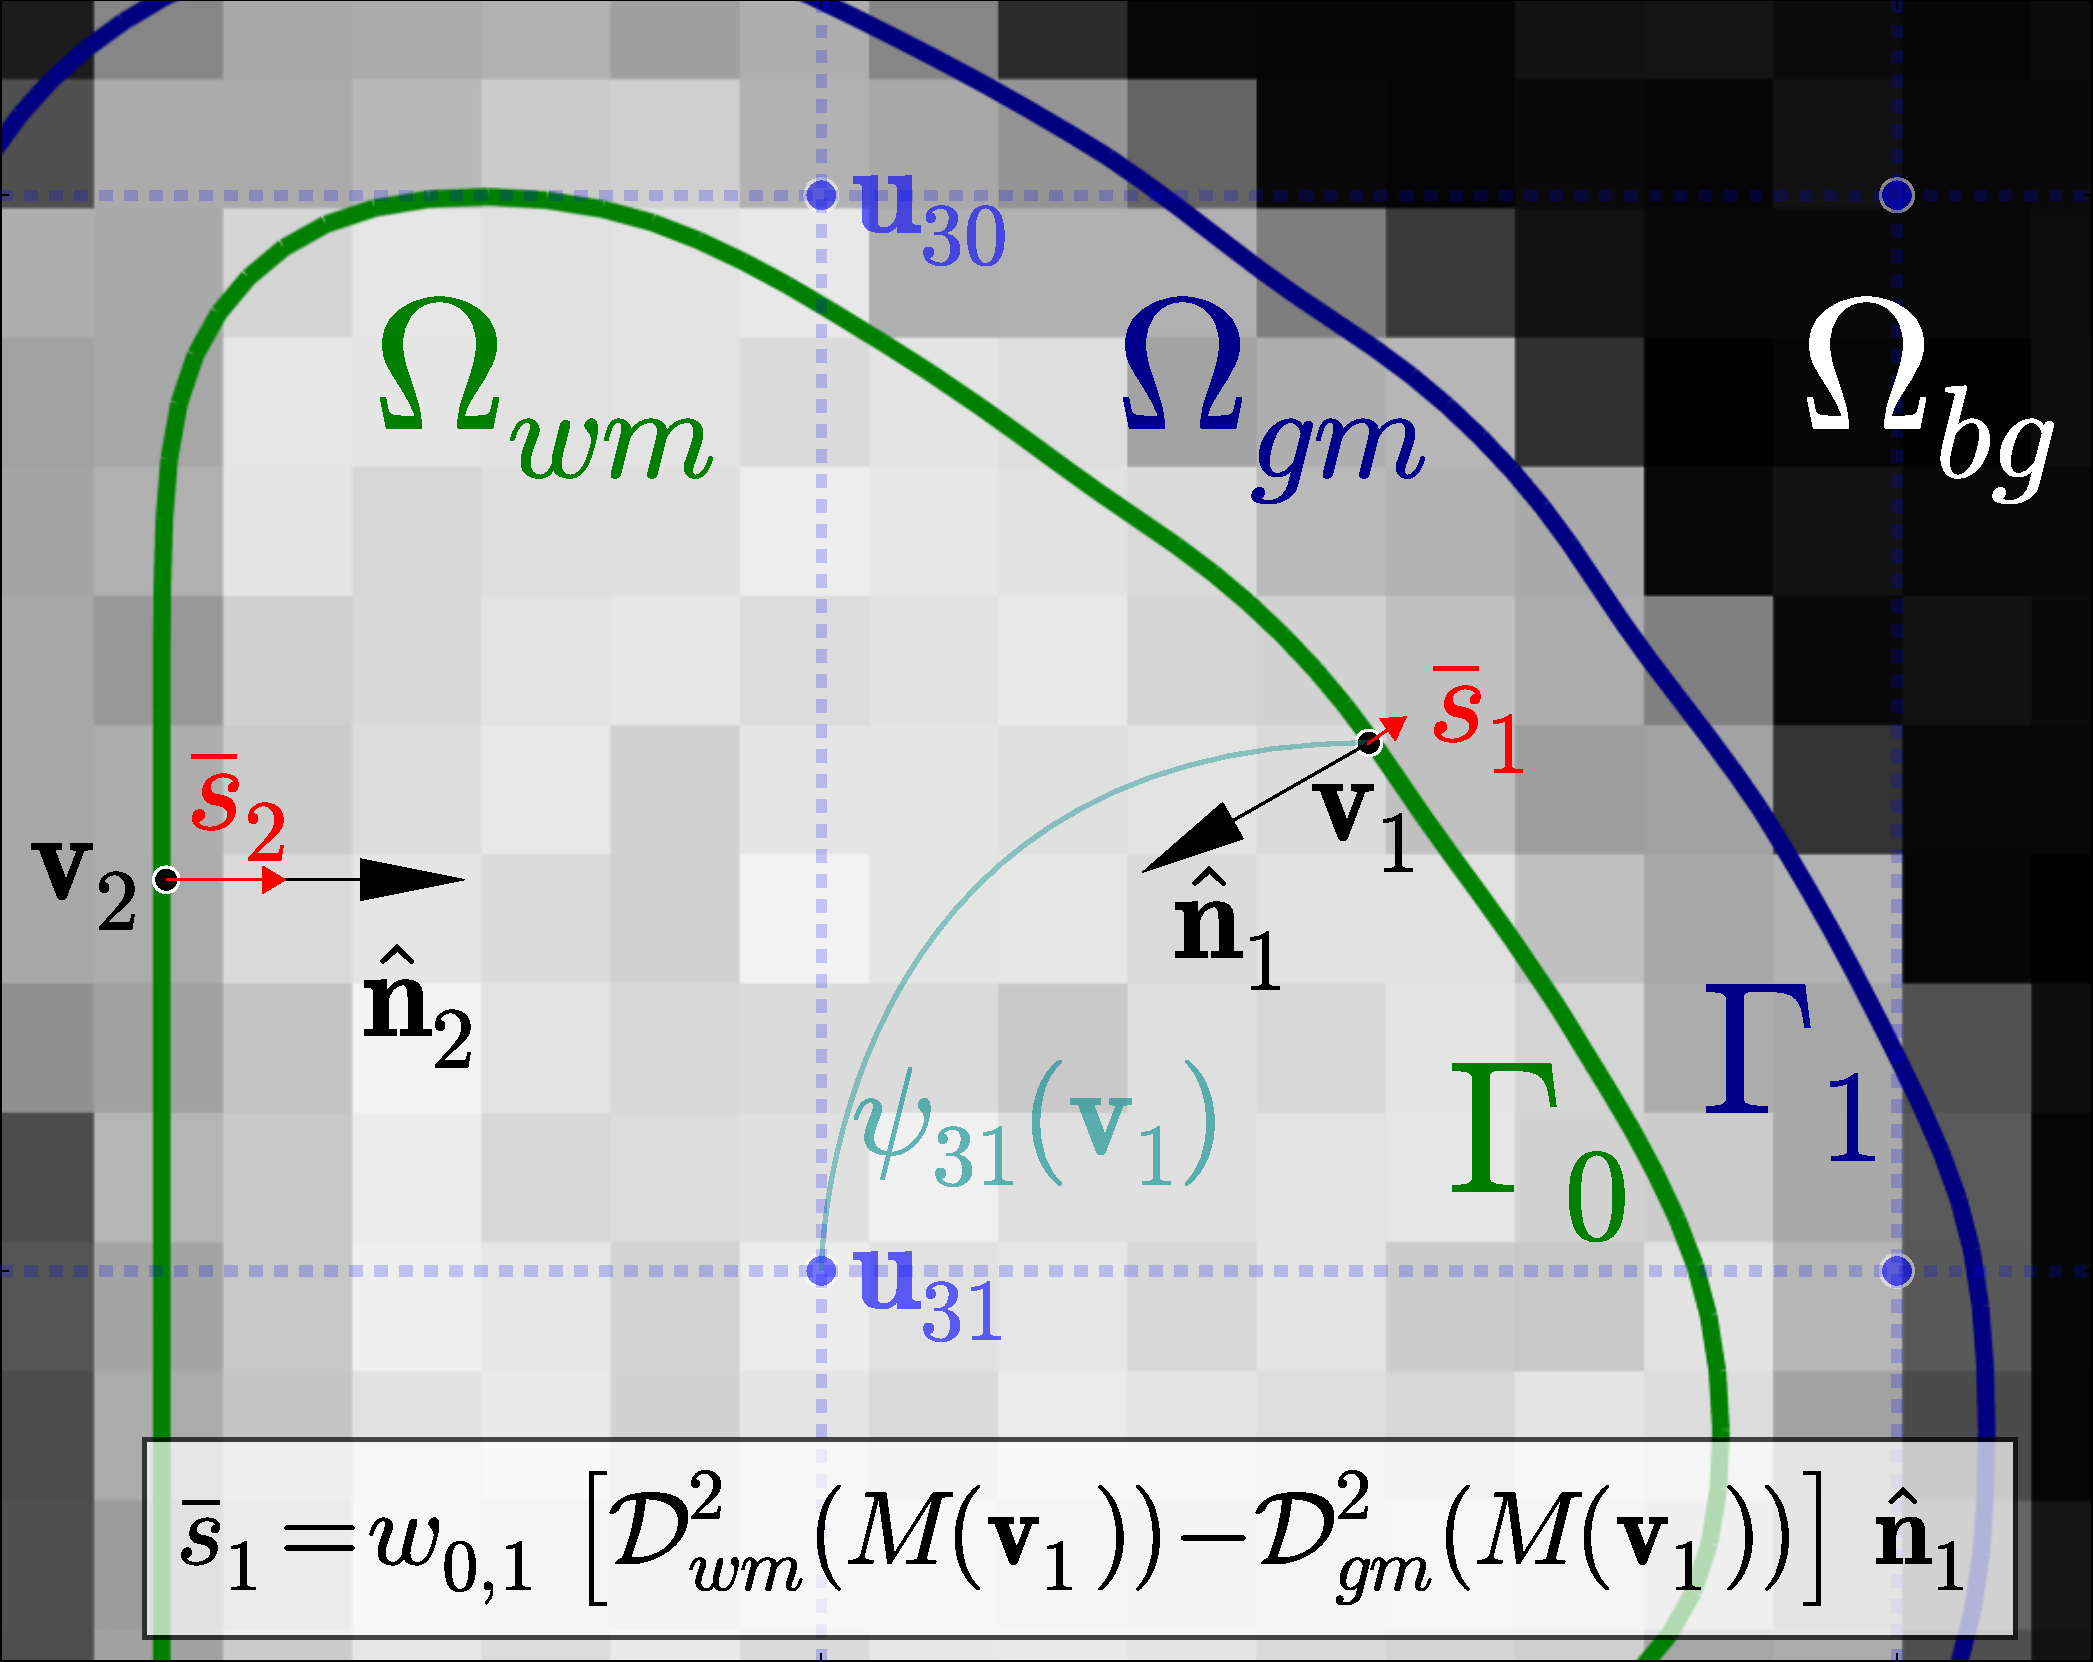
\includegraphics[width=\linewidth]{figure01}
	\caption{The active contours are defined as the interfacing surfaces of the competing
	  \glspl{roi} $\Omega_i$.
	They are represented in green and dark blue colors in this close-up.
	They iteratively evolve following their inward normals $\hat{n}_i$ at each vertex
	  $\vec{v}_i$ of the mesh.
	The gradient speeds $\bar{s}_i$ drive registration, and are computed as the disparity of data
    energies with respect to the two limiting regions of $M(\vec{v}_i)$, the features of the image
    $M$ in the location of vertex $\vec{v}_i$ (see \suppl{equation SM5}).
	In this figure, $\bar{s}_1$ is written in the lower
	  box, with $\Omega_{wm}$ being the inner limiting region, $\Omega_{gm}$ the outer region, and
    $w_{0,1}$ the relative area associated to vertex $\vec{v}_1$ with respect to
    the total area of surface $\Gamma_0$.
	% Finally, every $\bar{s}_i$ is associated with the control points $\vec{u}_k$ through
	%   the corresponding weights $\psi_k(\vec{v}_i)$ by Eq. \eqref{eq:gradient_wshape}.
	}\label{fig:method}
\end{figure}

\paragraph*{Deformation model}\label{sec:deformation_model}
Since the vertices of the surfaces $\{\vec{v}_i: \vec{v}_i \subset \gammaset \}_{i=1 \ldots N_v}$
  likely lay off-grid, it is required to derive $\vec{u}_i = \vec{u}(\vec{v}_i)$ from a discrete set of parameters
  $\{\vec{u}_k\}_{k=1 \ldots K}$.
Densification is achieved through a set of associated basis functions $\psi_k$ \eqref{eq:nodes_tfm}.
In our implementation, $\psi_k$ is chosen to be a tensor-product B-Spline kernel
  of degree 3.

  \begin{equation}
  \vec{v}_i' = \vec{v}_i + \vec{u}_i = \vec{v}_i + \sum_k \psi_k(\vec{r}) \: \vec{u}_k.
  \label{eq:nodes_tfm}
  \end{equation}


\paragraph*{Optimization}
\label{sec:gradient_descent}
To find the minimum of the energy functional \eqref{eq:energy},
  we propose a gradient-descent approach with respect to the underlying
  deformation field through the following \gls*{pde}:

  \begin{equation}
  \frac{\partial \vec{u}(\vec{r},t)}{\partial t} \propto - \frac{\partial E(\vec{u})}{\partial \vec{u}_k},
  \label{eq:general_gradient_descent}
  \end{equation}
%
  with $t$ being an artificial time parameter of the contour
  evolution, and $\vec{u}_k$ the parameters supporting the estimate
  $\hat{U}$ of the transformation at the current time point.
Let us assume that anisotropy is aligned with the imaging axes to simplify
  \eqref{eq:energy} into expression \eqref{eq:app_energy} of \ref{app:reg_term}
  and compute its derivative \eqref{eq:general_gradient_descent}:

  \begin{align}
  \frac{\partial E(\vec{u})}{\partial \vec{u}_k} &=
  \frac{ \partial }{\partial \vec{u}_k} \Big\{
  \underset{l}{\sum} \int_{\Omega_l} \mdist{f'}{l} \,d\vec{r} \, + % \notag\\ &+
  \int_{\Omega} \frac12 [ \boldsymbol{\alpha} \cdot \vec{u}^{\circ2}
  + \boldsymbol{\beta} \cdot (\nabla \vec{u})^{\circ2} ] \,d\vec{r}
  \Big\},
  \label{eq:gradient_descent}
  \end{align}
%
  where $\vec{u}^{\circ2} = \vec{u}^T \cdot \vec{u}$.
Then, the data and regularization terms are split and discretized to compute their
  derivatives.
The computation of the explicit shape gradients at each $\vec{v}_i'$ is described in \autoref{fig:method}.
Then, \eqref{eq:gradient_descent} can be reformulated as (see \suppl{equations SM6-SM12}):

  \begin{align}
  \frac{\partial E(\vec{u})}{\partial \vec{u}_k} &=
  \vec{g}_k  + \boldsymbol{\alpha} \cdot \vec{u}_k - \boldsymbol{\beta} \cdot (\Delta \vec{u}_k).
  \label{eq:final_gradient}
  \end{align}

Finally, to descend this gradient we establish a semi-implicit Euler scheme (see \suppl{section S1.3}),
  with a step size parameter $\delta$, that we solve in the spectral domain as follows:

  \begin{align}
  \vec{u}_k^{t+1} = \mathcal{F}^{-1}\left\{ \frac{\mathcal{F}\{\delta^{-1} \, \vec{u}_k^t - \vec{g}_k\} }%
                  {\mathcal{F}\{(\delta^{-1} + \boldsymbol{\alpha})\, I - \boldsymbol{\beta}\Delta\}} \right\},
  \label{eq:update_equation}
  \end{align}
  where $I$ denotes the identity operator.


\paragraph*{Implementation details, settings and convergence}
\label{sec:conv_report}
The \regseg{} tool includes a multiresolution strategy on the free-form deformation field.
Registration pyramids are created by setting the spacing between control points of the B-Spline basis
  functions for each level of the multiresolution.
This implementation detail, along with other features (as the sparse matrix approach
  to fast interpolation) and the main parameters 
  (such as $\delta$, $\boldsymbol{\alpha}$, $\boldsymbol{\beta}$, the B-Spline grid resolutions,
  target image smoothing, etc.) are discussed in the \suppl{section S1}.
The actual choices of parameter settings are publicly distributed with the source code of the experiments.
These final settings were manually obtained based on the feedback of post-registration convergence
  reports (as the one found in the \suppl{section S1.3}).
We release \regseg{} along with the tool for generating the convergence report.

\subsection{Evaluation protocol}\label{sec:evaluation_protocol}
In order to assess the performance of \regseg{}, we defined a general
  evaluation protocol:
1) Extraction of the set of undistorted surfaces $\gammaset_R$;
2) computation of a ground-truth field of displacements $U_{true}$ that is applied to
  generate warped images ($M$) to segment;
3) execution of \regseg{} with $\gammaset_R$ and the warped data as inputs; and
4) visual assessment and computation of error metrics.
How this protocol is adapted to the simulated phantoms and real data is covered in the
  following sections.

\subsection{Simulated phantoms}\label{sec:digital_phantoms}
The workflow to simulate the digital phantoms and assess
  \regseg{} on them is presented in \autoref{fig:evphantoms}.
A set of four binary objects (called ``box'', ``ball'', ``L'',
  and ``gyrus'') are generated combining binarization of
  analytical shapes and mathematical morphology.
The reference surfaces $\gammaset_R$ are extracted from the binary shapes
  using \emph{FreeSurfer} tools \citep{fischl_freesurfer_2012}.
The ground-truth distortion is generated with a chain of two displacement 
  fields supported by grids of B-Spline basis functions.
The coefficients of the basis functions are generated randomly for
  both levels in their three dimensions.
The three components of the displacements $\vec{u} = (u_d)$ 
  are bounded above by 40\% of the separation between control points
  at each level, to obtain diffeomorphic transforms
  after concatenation \citep{rueckert_diffeomorphic_2006}.
The first deformation field is intended to generate large warpings,
  with control points separated by 50.50mm along the three dimensions
  ($u_d\leq$ 20.20mm).
With the second warping, we look for a resulting field with smoothness
  close to the found in a typical distortion field of \gls*{dmri} data
  \citep{irfanoglu_susceptibility_2011}.
Therefore, the control points are separated 25.25mm ($u_d\leq$ 10.10mm).
Once the ground-truth deformation is generated, the original surfaces
  are warped interpolating the displacements field at each vertex.
The warped surfaces $\gammaset_\text{true}$ are binarized to generate tissue fractions
  in low (\isores[mm]{2.0}) and high (\isores[mm]{1.0}) resolution.
Using a \gls*{mr} simulator \citep{caruyer_phantomas_2014}, we synthesize
  \gls*{t1} (TE/TR= 10/1500ms) and \gls*{t2} images (TE/TR= 90/5000ms)
  corresponding to each phantom type, with two resolutions each
  (1.0mm and 2.0mm isotropic).
The field of view at both resolutions is \isores[mm]{100}.
Then, \regseg{} is applied to map $\gammaset_R$ into the warped phantoms to
  obtain the registered surfaces ($\hat{\gammaset}_{test}$).
% Simulations were corrupted with rician noise for a \gls*{snr} of 300.0.
To quantify the misregistration error, we compute the Hausdorff distance between
 $\hat{\gammaset}_{test}$ and $\gammaset_\text{true}$, using \citep{commandeur_vtk_2011}.

\begin{figure*}
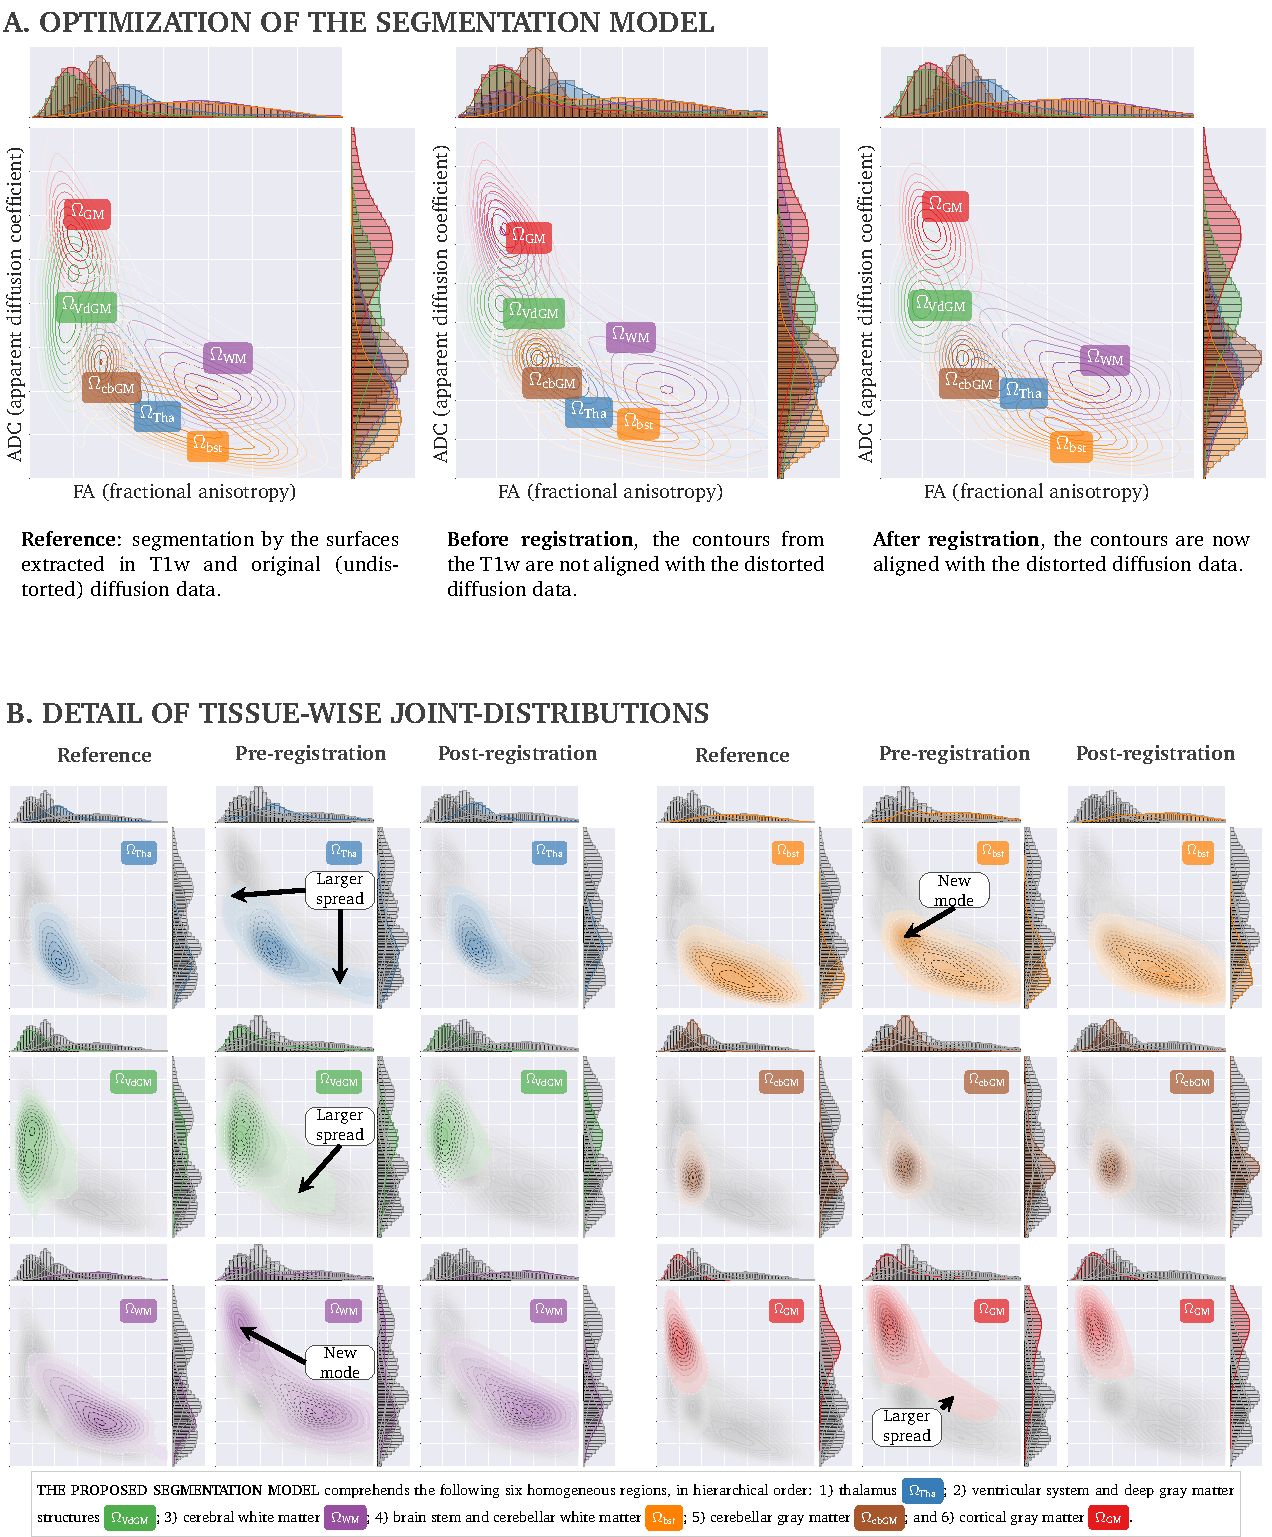
\includegraphics[width=\linewidth]{figure02}
\caption{The evaluation of \regseg{} on phantom data is performed with the presented instrumental workflow:
  1) The reference surfaces $\gammaset_R$ are triangularized meshes extracted from the four binary shapes (``box'', ``ball'', ``L'', ``gyrus'');
  2) A ground-truth displacement field is generated as described in \autoref{sec:digital_phantoms}, and applied to warp
      $\gammaset_R$, obtaining $\gammaset_\text{true}$;
  3) Once warped, $\gammaset_\text{true}$ are projected to the corresponding discrete 3D volume, and downsampled creating partial volume effects to two resolutions
     of \isores[mm]{2.0} and \isores[mm]{1.0}, producing sets of tissue fractions maps;
  4) The tissue fractions are fed to an \acrfull*{mr} simulator, generating \acrfull*{t1} and \acrfull*{t2} -like images at the
     two available resolutions;
  5) The \regseg{} is run, using the warped test images as moving multispectral-image and $\gammaset_R$ as shape-priors;
  6) Assessment of the agreement between the surfaces fitted with \regseg{} ($\hat{\gammaset}_{test}$) and $\gammaset_\text{true}$
     with automatically generated visual reports and computing the Hausdorff distance between corresponding surfaces.}\label{fig:evphantoms}
\end{figure*}


\subsection{Real datasets} %
\label{sec:human_connectome}
% 
The general experimental framework for the real datasets is presented in \autoref{fig:evworkflows}.
It extends our previous work \citep{esteban_simulationbased_2014} evaluating distortions
  on \gls*{dmri} phantoms.

\begin{figure*}
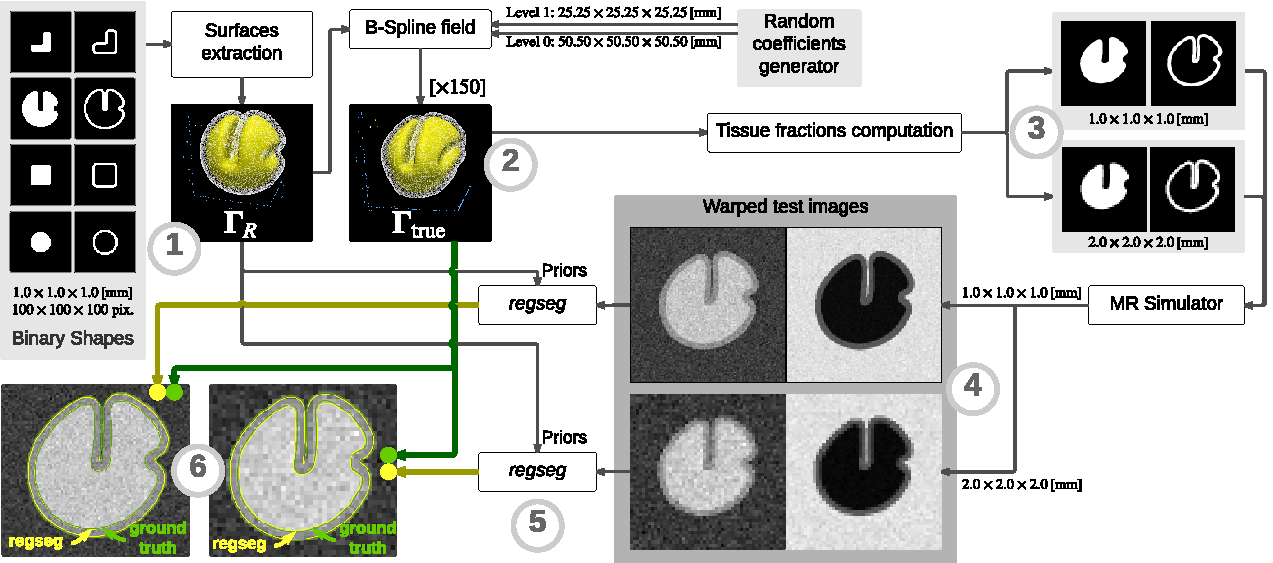
\includegraphics[width=\linewidth]{figure03}
\caption{Experimental workflow real data from the \acrfull*{hcp}.
  1) $\gammaset_R$ are extracted from the anatomical reference (\gls*{t1} image).
  2) To operate as ground truth, we generate a plausible-synthetic distortion $U_{true}$
    from the fieldmap using \eqref{eq:fieldmap}.
  3) The \gls*{dmri} data are warped using $U_{true}$ to reproduce the effects of real
    susceptibility-derived distortions.
  Target diffusion scalars (\gls*{fa} and \gls*{adc}) are computed on the distorted data and
    stacked to feed the multivariate input required by \regseg{}.
  4) the method is run, obtaining a $U_{test} = \hat{U}_{true}$, the estimation of
    the ground-truth deformation.
  5) Results are visually and quantitatively evaluated.}\label{fig:evworkflows}
\end{figure*}


\paragraph*{Data}
For the evaluation of \regseg{} on real \gls*{dmri} data of human brains,
  we collected 16 subjects from the \gls*{hcp} database.
The original acquisitions are released within ``unprocessed'' packages, and
  the ``minimally preprocessed'' are corrected for artifacts, brain-extracted
  and spatially normalized, along with some results of the standard processing
  pipeline of \emph{FreeSurfer}.
We refer the reader to \citep{essen_human_2012} for exact details about acquisition
  parameters, and \citep{glasser_minimal_2013} for the preprocessing issues.
The datasets comprehend a large set of images, containing \gls*{t1}, \gls*{t2} and
  multi-shell \gls*{dmri} images.

\begin{figure}
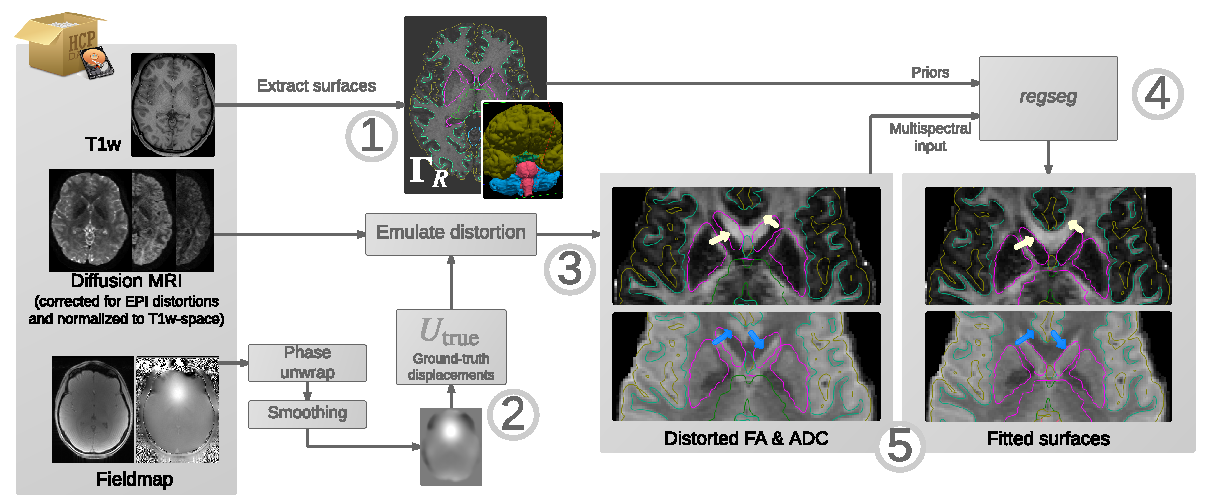
\includegraphics[width=\linewidth]{figure04}
\caption{Segmentation model defined by the homogeneous regions $\Omega_i$ in which
  the image to be segmented is partitioned by the theoretical projection 
  ($\gammaset_{true}$) of $\gammaset_R$ into $M$.
The plot represents a kernel density estimation of the location and spread of
  each region $\Omega_i$ in the bivariate feature space of $M$, comprising 
  the \gls*{fa} and \gls*{adc} maps.
On top and right margins the marginal distributions of $\Omega_i$ are also plotted for
  the \gls*{fa} and \gls*{adc}, respectively.
}\label{fig:model}
\end{figure}

\paragraph*{Segmentation model}
Based on our experience \citep{esteban_brain_2012} and previous studies \citep{ennis_orthogonal_2006},
  we define the moving image as a stack of the \gls*{fa} and \gls*{adc} maps derived
  from \gls*{dmri} data.
After evaluating several alternative models, we empirically defined a partition \omegaset{}
  into the following six regions:
  1) the thalamus ($\Omega_{Tha}$);
  2) the ventricular system and deep \gls*{gm} structures ($\Omega_{VdGM}$);
  3) the cerebral \gls*{wm} ($\Omega_{WM}$);
  4) the brain stem and cerebellar \gls*{wm} ($\Omega_{bst}$);
	5) the cerebellar \gls*{gm} ($\Omega_{cbGM}$); and
	6) the cortical \gls*{gm} ($\Omega_{GM}$).
Using tools of \emph{FreeSurfer}, and the appropriate selections of labels in the 
  \emph{aparc} segmentation released with the \gls*{hcp} data, the $\gammaset_R$ set of
  reference surfaces is extracted.
The segmentation model corresponding to this partition is depicted in \autoref{fig:model},
  and discussed with finer detail in \suppl{section S4}.

\paragraph*{Ground-truth generation}
Realistic deformation is achieved generating displacements fields that meet the theoretical
  properties of distortion \citep{jezzard_correction_1995}.
The displacements along the \gls*{pe} axis of the \gls*{dmri} image are related to the local
  deviation of the field $\Delta B_0(\vec{r})$ from its nominal value $B_0$ as follows:

  \begin{equation}
  u_\text{PE} = \frac{\gamma \, T_{acq}\, s_\text{PE}}{2\pi}\Delta B_0(\vec{r})\text{ [mm]},
  \label{eq:fieldmap}
  \end{equation}
%
where $\gamma$ is the gyromagnetic ratio, $T_{acq}$ is the readout time, and
  $s_\text{PE}$ is the pixel size along \gls*{pe}.
Certain \gls*{mr} sequences are designed to estimate $\Delta B_0$, obtaining
  the so-called fieldmap.
We derive the deformation $U_{true}$ from the fieldmap image released with
  the corresponding packages of each dataset from the \gls*{hcp}.
The fieldmap is unwrapped\footnote{fieldmaps are phase maps, clipped in the interval
  of $[-\pi, \pi)$ [rads] or [rads/s].} and smoothed before applying \eqref{eq:fieldmap}.
Then, the original \gls*{dmri} is warped using the resulting displacements field and fed into
  a pipeline that process the corresponding \gls*{dti} and computes the derived scalars of
  interest (\gls*{fa} and \gls*{adc}) using \emph{MRtrix} \citep{tournier_mrtrix_2012}.

\paragraph*{Metric assessment}
Preliminarily, we investigated the aptness of the segmentation model.
For five test datasets, we uniformly sampled the space of distortions
  $\hat{U} = \epsilon \cdot U_{true} = \vec{r} + \epsilon \, u_\text{PE}$
  (with $\epsilon \in [-1.1, 1.1]$ and $u_\text{PE}$ from \eqref{eq:fieldmap}),
  and evaluated the data-term of the cost function \eqref{eq:energy}.
The metric consistently displayed its minimum at the ground-truth location ($\epsilon=0.0$)
  for all the cases (\suppl{Figure S2}).

\paragraph*{Cross-comparison}
A dual workflow to the general evaluation framework of \autoref{fig:evworkflows}
  integrates the alternate \gls*{t2b} registration scheme.
We reproduced the solution and settings provided with \emph{ExploreDTI}
  \citep{leemans_exploredti_2009}, a widely used toolkit for tractography analysis of
  \gls*{dti}.
\emph{ExploreDTI}, internally uses \emph{elastix} \citep{klein_elastix_2010} to
  perform registration.

\paragraph*{Error measurement}\label{sec:experiments_evaluation}
Since the distortions only happen along the \gls*{pe} axis of the image, we compute the
  \gls*{swindex} as the area-weighted distance between corresponding vertices of 
  $\gammaset_{true}$ and their estimation by the method under test $\hat{\gammaset}_{test}$:

  \begin{equation}
  sWI = \frac{1}{\sum_i a_i} \sum\limits_i^{N_V} a_i\,\|
  \vec{v}_i - \hat{\vec{v}}_i \|,
  \label{eq:swindex}
  \end{equation}
%
  where $\vec{v}_i \subset \gammaset_\text{true}$ are the locations of the total $N_V$ vertices,
  and $\hat{\vec{v}}_i \subset \hat{\gammaset}_{test}$ are the locations
  recovered corresponding to $\vec{v}_i$.
In practice, we report the \gls*{swindex} only for three surfaces of interest crucial in whole-brain
  tractography.
These three surfaces delineate the following regions in the model: $\Omega_{VdGM}$, $\Omega_{WM}$ and $\Omega_{GM}$.